% Para utilizar este template siga o tutorial disponível em http://www.biblioteca.ufc.br/wp-content/uploads/2015/09/tutorial-sharelatex.pdf

%%%%%%%%%%%%%%%%%%%%%%%%%%%%%%%%%%%%%%%%%%%%%%%%%%%%%%%
%% Você deve criar uma conta no Overleaf. Depois,    %%
%% vá nas opções no canto esquerdo superior da tela  %%
%% e clique em "Copiar Projeto". Dê um novo nome pa- %%
%% ra o projeto.                                     %%
%%                                                   %%
%% Os principais desenvolvedores deste template são: %%
%%                                                   %%
%%            Ednardo Moreira Rodrigues              %%
%%       (Doutor em Engenharia Elétrica - UFC)       %%
%%                      &                            %%
%%            Alan Batista de Oliveira               %%
%%           (Engenheiro Eletricista - UFC)          %%
%%                                                   %%
%% Consultoria Bibliotecária                         %%
%%                                                   %%
%%  Versão 2016 - ShareLaTeX:                        %%
%%                                                   %%
%% - Francisco Edvander Pires Santos;                %%
%% - Juliana Soares Lima;                            %%
%% - Izabel Lima dos Santos;                         %%
%% - Kalline Yasmin Soares Feitosa;                  %%
%% - Eliene Maria Vieira de Moura.                   %%
%%
%%  Versão 2019 - Overleaf:
%%
%%  Biblioteca de Ciências Humanas:
%% - Francisco Edvander Pires Santos;                %%
%% - Juliana Soares Lima;                            %%
%% - Eliene Maria Vieira de Moura;                   %%
%% - Edmundo Moreira de Sousa Filho.                 %%
%%                                                   %%
%% Biblioteca da FEAAC:                              %%
%% - Izabel Lima dos Santos;                         %%
%% - Kalline Yasmin Soares Feitosa;                  %%
%% - Kleber Lima dos Santos.                         %%
%%                                                   %%
%%  Biblioteca do Curso de Física:                   %%
%% - Aline Rodrigues de Lima Mendes;                 %%
%% - Maria de Jesus Silva dos Santos.                %%
%%                                                   %%
%%  Biblioteca Central do Campus do Pici:            %%
%% - Raquel da Silva Nascimento.                     %%
%%                                                   %%
%% Colaboradores                                     %%
%%                                                   %%
%% -Andrei Bosco Bezerra Torres                      %%
%% (Professor - Sistemas e Mídias Digitais -         %%
%% Instituto Universidade Virtual - UFC)             %%
%% Tiago ALves Lima                                  %%
%% (Aluno de Mestrado em Eng. Elétrica)              %%
%%                                                   %%
%% Grande parte do trabalho foi adaptado do template %%
%% da UECE elaborado por:                            %%
%% Thiago Nascimento  (UECE)                         %%
%% Project available on:                             %%
%% https://github.com/thiagodnf/uecetex2             %%
%%                                                   %%
%% "Dúvidas, esclarecimentos ou sugestões podem ser  %%
%% enviadas para o seguinte e-mail:                  %%
%%                                                   %%
%%             atendimentobch@ufc.br                 %%
%%                                                   %%
%% As últimas atualizações estão descritas no inicio %%
%% do arquivo "README.md".                           %%
%%                                                   %%
%%%%%%%%%%%%%%%%%%%%%%%%%%%%%%%%%%%%%%%%%%%%%%%%%%%%%%%

\documentclass[
    a4paper,          % Tamanho da folha A4
    12pt,             % Tamanho da fonte 12pt
    chapter=TITLE,    % Todos os capitulos devem ter caixa alta
    section=Title,    % Todas as secoes devem ter caixa alta somente na primeira letra
    subsection=Title, % Todas as subsecoes devem ter caixa alta somente na primeira letra
    oneside,          % Usada para impressao em apenas uma face do papel
    english,          % Hifenizacoes em ingles
    spanish,          % Hifenizacoes em espanhol
    brazil,           % Ultimo idioma eh o idioma padrao do documento
    fleqn             % Comente esta linha se quiser centralizar as equacoes. Comente também a linha 65 abaixo
]{abntex2}

% Para utilizar este template siga o tutorial disponível em http://www.biblioteca.ufc.br/wp-content/uploads/2015/09/tutorial-sharelatex.pdf

%%%%%%%%%%%%%%%%%%%%%%%%%%%%%%%%%%%%%%%%%%%%%%%%%%%%%%%
%% Você deve criar uma conta no Overleaf. Depois,    %%
%% vá nas opções no canto esquerdo superior da tela  %%
%% e clique em "Copiar Projeto". Dê um novo nome pa- %%
%% ra o projeto.                                     %%
%%                                                   %%
%% Os principais desenvolvedores deste template são: %%
%%                                                   %%
%%            Ednardo Moreira Rodrigues              %%
%%       (Doutor em Engenharia Elétrica - UFC)       %%
%%                      &                            %%
%%            Alan Batista de Oliveira               %%
%%           (Engenheiro Eletricista - UFC)          %%
%%                                                   %%
%% Revisão:                                          %%
%%                                                   %%
%% - Francisco Edvander Pires Santos;                %%
%% - Juliana Soares Lima;                            %%
%% - Izabel Lima dos Santos;                         %%
%% - Kalline Yasmin Soares Feitosa.                  %%
%% - Eliene Maria Vieira de Moura;                   %%
%%                                                   %%
%% Colaboradores                                     %%
%%                                                   %%
%% -Andrei Bosco Bezerra Torres                      %%
%% (Professor - Sistemas e Mídias Digitais -         %%
%% Instituto Universidade Virtual - UFC)             %%
%% Tiago ALves Lima                                  %%
%% (Aluno de Mestrado em Eng. Elétrica)              %%
%%                                                   %%
%% Grande parte do trabalho foi adaptado do template %%
%% da UECE elaborado por:                            %%
%% Thiago Nascimento  (UECE)                         %%
%% Project available on:                             %%
%% https://github.com/thiagodnf/uecetex2             %%
%%                                                   %%
%% "Dúvidas, esclarecimentos ou sugestões podem ser  %%
%% enviadas para o seguinte e-mail:                  %%
%%                                                   %%
%%             atendimentobch@ufc.br                 %%
%%                                                   %%
%% As últimas atualizações estão descritas no inicio %%
%% do arquivo "README.md".                           %%
%%                                                   %%
%%%%%%%%%%%%%%%%%%%%%%%%%%%%%%%%%%%%%%%%%%%%%%%%%%%%%%%

% Importações de pacotes
\usepackage[utf8]{inputenc}                         % Acentuação direta
\usepackage[T1]{fontenc}                            % Codificação da fonte em 8 bits
\usepackage{graphicx}                               % Inserir figuras
\usepackage{amsfonts, amssymb, amsmath}             % Fonte e símbolos matemáticos
\usepackage{booktabs}                               % Comandos para tabelas
\usepackage{verbatim}                               % Texto é interpretado como escrito no documento
\usepackage{multirow, array}                        % Múltiplas linhas e colunas em tabelas
\usepackage{indentfirst}                            % Endenta o primeiro parágrafo de cada seção.
\usepackage{listings}                               % Utilizar codigo fonte no documento
\usepackage[table,xcdraw]{xcolor}
\usepackage{xcolor}
\usepackage{microtype}                              % Para melhorias de justificação?
\usepackage[portuguese,ruled,lined]{algorithm2e}    % Escrever algoritmos
\usepackage{algorithmic}                            % Criar Algoritmos
%\usepackage{float}                                 % Utilizado para criação de floats
\usepackage{amsgen}
\usepackage{lipsum}                                 % Usar a simulação de texto Lorem Ipsum
%\usepackage{titlesec}                              % Permite alterar os títulos do documento
\usepackage{tocloft}                                % Permite alterar a formatação do Sumário
\usepackage{etoolbox}                               % Usado para alterar a fonte da Section no Sumário
\usepackage[nogroupskip,nonumberlist]{glossaries}   % Permite fazer o glossario

\usepackage[font=singlespacing,format=plain,justification=justified,skip=0pt,singlelinecheck = false]{caption}            % Altera o comportamento da tag caption

\usepackage[alf, abnt-emphasize=bf, recuo=0cm, abnt-etal-cite=2, abnt-etal-list=0, abnt-etal-text=it]{abntex2cite}  % Citações padrão ABNT
%\usepackage[bottom]{footmisc}                      % Mantém as notas de rodapé sempre na mesma posição
%\usepackage{times}                                 % Usa a fonte Times
%%%%%%%%%%%%%%%%%%% AVISO %%%%%%%%%%%%%%%%%%%%%%%%%%%%%%%%%%%%%%%%
%descomente as duas linhas abaixo para alterar o texto de Times New Roman para Arial:

%\usepackage{helvet}
%\renewcommand{\familydefault}{\sfdefault}  % Usa a fonte Arial
%%%%%%%%%%%%%%%%%%%%%%%%%%%%%%%%%%%%%%%%%%%%%%%%%%%%%%%%%%%%%%%%%%

\usepackage{mathptmx}         % Usa a fonte Times New Roman			%\usepackage{lmodern}         % Usa a fonte Latin Modern
%\usepackage{subfig}          % Posicionamento de figuras
%\usepackage{scalefnt}        % Permite redimensionar tamanho da fonte
%\usepackage{color, colortbl} % Comandos de cores
%\usepackage{lscape}          % Permite páginas em modo "paisagem"
%\usepackage{ae, aecompl}     % Fontes de alta qualidade
%\usepackage{picinpar}        % Dispor imagens em parágrafos
%\usepackage{latexsym}        % Símbolos matemáticos
%\usepackage{upgreek}         % Fonte letras gregas
\usepackage{appendix}         % Gerar o apendice no final do documento
\usepackage{paracol}          % Criar paragrafos sem identacao
\usepackage{lib/ufctex}	      % Biblioteca com as normas da UFC para trabalhos academicos
\usepackage{pdfpages}         % Incluir pdf no documento
\usepackage{amsmath}          % Usar equacoes matematicas


\makeglossaries% Organiza e gera a lista de abreviaturas, simbolos e glossario
\makeindex     % Gera o Indice do documento


\setlength{\mathindent}{0pt} %Complementa o alinhamento de equações para totalmente a esquerda.

%%%%%%%%%%%%%%%%%%%%%%%%%%%%%%%%%%%%%%%%%%%%%%%%%%%%%
%%                     ATENCAO                     %%
%%%%%%%%%%%%%%%%%%%%%%%%%%%%%%%%%%%%%%%%%%%%%%%%%%%%%
%  Qual e o nivel do trabalho academico que voce esta
% escrevendo? Retire o simbolo "%" apenas de um dos
% quatro topicos abaixo refente ao nível do seu traba
% -lho.

\trabalhoacademico{tccgraduacao}
%\trabalhoacademico{tccespecializacao}
%\trabalhoacademico{dissertacao}
%\trabalhoacademico{tese}

%%%%%%%%%%%%%%%%%%%%%%%%%%%%%%%%%%%%%%%%%%%%%%%%%%%%%

% Define se o trabalho e uma qualificacao
% Coloque 'nao' para versao final do trabalho

\ehqualificacao{nao}

% Remove as bordas vermelhas e verdes do PDF gerado
% Coloque 'sim' pare remover

\removerbordasdohyperlink{sim}

% Adiciona a cor Azul a todos os hyperlinks

\cordohyperlink{nao}

%%%%%%%%%%%%%%%%%%%%%%%%%%%%%%%%%%%%%%%%%%%%%%%%%%%%%
%%         Informacao sobre a instituicao          %%
%%%%%%%%%%%%%%%%%%%%%%%%%%%%%%%%%%%%%%%%%%%%%%%%%%%%%

\ies{Universidade Federal do Ceará}
\iessigla{UFC}
\centro{Campus de Sobral}
\departamento{Departamento de Computação}

%%%%%%%%%%%%%%%%%%%%%%%%%%%%%%%%%%%%%%%%%%%%%%%%%%%%%
%%        Informacao para TCC de Graduacao         %%
%%%%%%%%%%%%%%%%%%%%%%%%%%%%%%%%%%%%%%%%%%%%%%%%%%%%%

\graduacaoem{Engenharia da Computação}
\habilitacao{bacharel} % Ou licenciado(a)

% AVISO: Caso necessario alterar o texto de apresenta-
% cao da Especializacao, ir a pasta "lib", arquivo
% "ufctex.sty" na linha 502.


%%%%%%%%%%%%%%%%%%%%%%%%%%%%%%%%%%%%%%%%%%%%%%%%%%%%%
%%     Informacao para TCC de Especializacao       %%
%%%%%%%%%%%%%%%%%%%%%%%%%%%%%%%%%%%%%%%%%%%%%%%%%%%%%

\especializacaoem{Yyyyyyyyy}

% AVISO: Caso necessario alterar o texto de apresenta-
% cao da Especializacao, ir a pasta "lib", arquivo
% "ufctex.sty" na linha 507.

%%%%%%%%%%%%%%%%%%%%%%%%%%%%%%%%%%%%%%%%%%%%%%%%%%%%%
%%         Informacao para Dissertacao             %%
%%%%%%%%%%%%%%%%%%%%%%%%%%%%%%%%%%%%%%%%%%%%%%%%%%%%%

\programamestrado{Programa de Pós-Graduação em Xxxxxxx}
\nomedomestrado{Mestrado Acadêmico em Xxxxxxx}
\mestreem{Engenharia Xxxxxx}
\areadeconcentracaomestrado{Engenharia Xxxxxx}

% AVISO: Caso necessario alterar o texto de apresenta-
% cao da dissertacao, ir a pasta "lib", arquivo
% "ufctex.sty" na linha 511.

%%%%%%%%%%%%%%%%%%%%%%%%%%%%%%%%%%%%%%%%%%%%%%%%%%%%%
%%               Informação para Tese              %%
%%%%%%%%%%%%%%%%%%%%%%%%%%%%%%%%%%%%%%%%%%%%%%%%%%%%%

\programadoutorado{Programa de Pós-Graduação em Xxxxxx}
\nomedodoutorado{Doutorado em Xxxxxxx}
\doutorem{Engenharia Xxxxxx}
\areadeconcentracaodoutorado{Engenharia Xxxxxxx}

% AVISO: Caso necessario alterar o texto de apresenta-
% cao da tese, ir a pasta "lib", arquivo "ufctex.sty"
% na linha 515.

%%%%%%%%%%%%%%%%%%%%%%%%%%%%%%%%%%%%%%%%%%%%%%%%%%%%%
%%      Informacoes relacionadas ao trabalho       %%
%%%%%%%%%%%%%%%%%%%%%%%%%%%%%%%%%%%%%%%%%%%%%%%%%%%%%

\autor{Manoel Vilela Machado Neto}
\titulo{Segmentação Semi-Supervisionada de Imagens através de
Dinâmicas Coletivas em Redes Complexas}
\data{2021}
\local{Sobral}

% Exemplo: \dataaprovacao{01 de Janeiro de 2012}
\dataaprovacao{}

%%%%%%%%%%%%%%%%%%%%%%%%%%%%%%%%%%%%%%%%%%%%%%%%%%%%%
%%           Informação sobre o Orientador         %%
%%%%%%%%%%%%%%%%%%%%%%%%%%%%%%%%%%%%%%%%%%%%%%%%%%%%%

\orientador{Prof. Dr. Jarbas Joaci de Mesquita Sá Junior}
\orientadories{Universidade Federal do Ceará (UFC)}
\orientadorcentro{Centro de Ciências e Tecnologia (CCT)}
\orientadorfeminino{nao} % Coloque 'sim' se for do sexo feminino

%%%%%%%%%%%%%%%%%%%%%%%%%%%%%%%%%%%%%%%%%%%%%%%%%%%%%
%%          Informação sobre o Coorientador        %%
%%%%%%%%%%%%%%%%%%%%%%%%%%%%%%%%%%%%%%%%%%%%%%%%%%%%%

% Deixe o nome do coorientador em branco para remover do documento

\coorientador{Prof. Dr. Filipe A. N. Verri}
\coorientadories{Instituto Tecnológico da Aeronaútica (ITA)}
\coorientadorcentro{Divisão de Ciência da Computação (IEC)}
\coorientadorfeminino{nao} % Coloque 'sim' se for do sexo feminino

%%%%%%%%%%%%%%%%%%%%%%%%%%%%%%%%%%%%%%%%%%%%%%%%%%%%%
%%              Informação sobre a banca           %%
%%%%%%%%%%%%%%%%%%%%%%%%%%%%%%%%%%%%%%%%%%%%%%%%%%%%%

% Atenção! Deixe em branco o nome do membro da banca para remover da folha de aprovacao

% Exemplo de uso:
% \membrodabancadois{Prof. Dr. Fulano de Tal}
% \membrodabancadoisies{Universidade Federal do Ceará - UFC}


% \membrodabancadois{Prof. Dr. Xxxxxxx Xxxxxx Xxxxxxx}
% \membrodabancadoiscentro{Faculdade de Filosofia Dom Aureliano Matos (FAFIDAM)}
% \membrodabancadoisies{Universidade do Membro da Banca Dois (SIGLA)}
% \membrodabancatres{Prof. Dr. Xxxxxxx Xxxxxx Xxxxxxx}
% \membrodabancatrescentro{Centro de Ciências e Tecnologia (CCT)}
% \membrodabancatresies{Universidade do Membro da Banca Três (SIGLA)}
% \membrodabancaquatro{Prof. Dr. Xxxxxxx Xxxxxx Xxxxxxx}
% \membrodabancaquatrocentro{Centro de Ciências e Tecnologia (CCT)}
% \membrodabancaquatroies{Universidade do Membro da Banca Quatro (SIGLA)}
% \membrodabancacinco{Prof. Dr. Xxxxxxx Xxxxxx Xxxxxxx}
% \membrodabancacincocentro{Teste}
% \membrodabancacincoies{Universidade do Membro da Banca Cinco (SIGLA)}
% \membrodabancaseis{Prof. Dr. Xxxxxxx Xxxxxx Xxxxxxx}
% \membrodabancaseiscentro{}
% \membrodabancaseisies{Universidade do Membro da Banca Seis (SIGLA)}
%
\begin{document}

	% Elementos pré-textuais
	\imprimircapa
	\imprimirfolhaderosto{}
	%\imprimirfichacatalografica{1-pre-textuais/ficha-catalografica}
	%\imprimirerrata{elementos-pre-textuais/errata}
	%\imprimirfolhadeaprovacao
	%\imprimirdedicatoria{1-pre-textuais/dedicatoria}
	%\imprimiragradecimentos{1-pre-textuais/agradecimentos}
	%\imprimirepigrafe{1-pre-textuais/epigrafe}
	%\imprimirresumo{1-pre-textuais/resumo}
	%\imprimirabstract{1-pre-textuais/abstract}
    % Se você comentar esta linha o título da lista fica: LISTA DE ILUSTRAÇÕES
	\renewcommand*\listfigurename{Lista de Figuras}
	%\imprimirlistadeilustracoes
	%\imprimirlistadetabelas
	%\imprimirlistadequadros
	%\imprimirlistadealgoritmos
	%\imprimirlistadecodigosfonte
	%\imprimirlistadeabreviaturasesiglas
	%\imprimirlistadesimbolos{1-pre-textuais/lista-de-simbolos}
	\imprimirsumario

	\setcounter{table}{0}% Deixe este comando antes da primeira tabela.

	%Elementos textuais
	\textual
	\chapter{INTRODUÇÃO}\label{cap:introducao}

Sistemas de segmentação de imagens têm se tornado populares em
variadas aplicações, como, por exemplo, a área de edição de imagem,
diagnósticos médicos e parte da visão computacional necessária pra
reconhecimento de objetos. Entre esses motivos e outros, essa área tem
uma relevância científica alta considerando a situação social,
tecnológica e econômica que é vivida no século XXI.\@

A segmentação de uma imagem pode ser feita manualmente por um anotador
humano marcando as linhas delineadoras de um objeto. Por outro lado,
são conhecido algoritmos variados para segmentação de imagens baseados
em aprendizagem de máquina, que através de exemplos de segmentação
fornecidos para treinamento é possível inferir a segmentação de novas imagens.

Na Figura~\ref{fig:image-segmentation-types} é apresentado um quadro
comparativo de operações em uma imagem com balões, incluindo os tipos
de segmentação de imagens conhecidos: semântica e instância. Na
segmentação semântica o objetivo é segmentar apenas os mesmos tipos de
objetos como o mesmo rótulo, na segmentação por instância, cada balão
é visto como a mesma classe de balão mas com rótulos associados diferentes.

\begin{figure}[h!]
        \captionsetup{width=16cm}
		\Caption{\label{fig:image-segmentation-types}
Comparação de tipos de segmentação de imagem: por semântica e instância
}
		\centering
		\UFCfig{}{\fbox{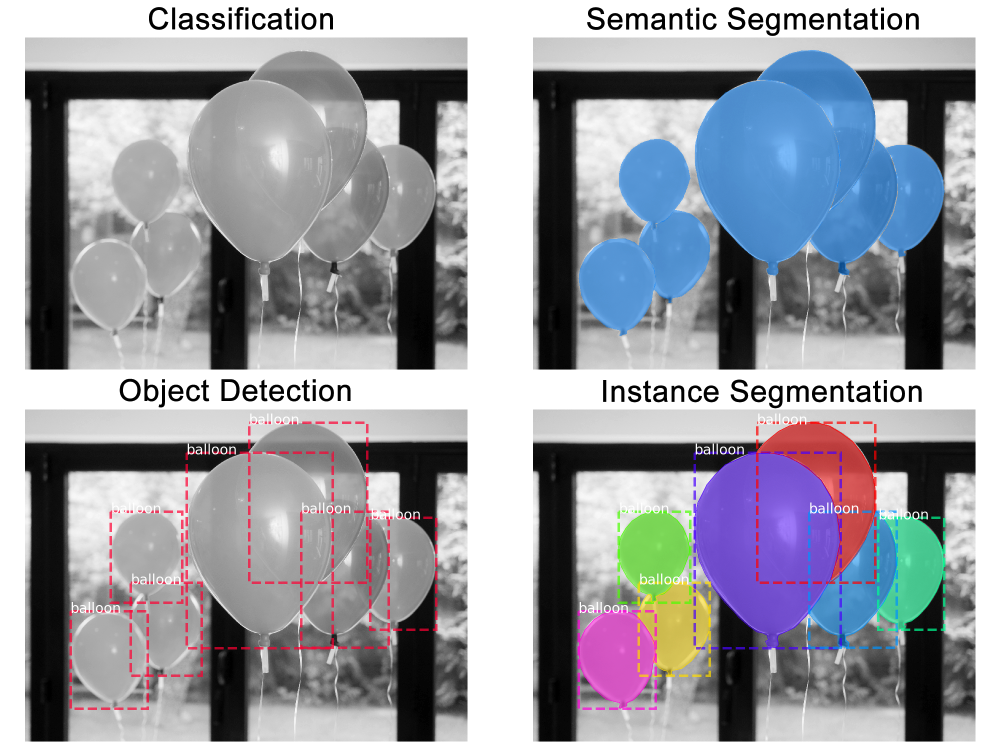
\includegraphics[width=16cm]{figuras/image-segmentation-types}}}{\Fonte{\citeonline{MediumInstanceSegmentation2019}}}
\end{figure}


Entre os tipos de aprendizagem de máquina, para segmentação de imagens
semântica é selecionada neste trabalho especificamente a aprendizagem
semi-supervisionada transdutiva\footnote{mais informações na
seção~\ref{sec:teorica-aprendizado-semi-supervisionado}}. A
aprendizagem semi-supervisionada é uma categoria que realiza o
aprendizado com poucas rotulações e maior parte dos dados não são
rotulados. Outras categorias de aprendizado de máquina como
supervisionada possui no treinamento uma base totalmente rotulada
enquanto a aprendizagem não-supervisionada não possui rótulo algum
(exemplo: K-means). Ao considerar a dificuldade de conseguir dados
rotulados por humanos em ambientes de uso por especialistas, como imagens
médicas e ferramentas de edição de imagem, a abordagem
semi-supervisionada se demonstra interessante por precisar de poucos
dados rotulados, mas ainda existir uma anotação com viés do
especialista interessado (médico, editor).


Os três principais algoritmos clássicos de segmentação de imagem podem
ser citados: \textit{Region-Based Segmentation}; \textit{Edge Detection
  Segmentation}; \textit{Segmentation based on Clustering}
~\cite{ImageSegmentationTechniques1985}. Cada uma dessas técnicas
possui limitações conhecidas, e entre elas é possível mencionar: haver
muitos objetos na imagem pode dificultar a segmentação; tempo
computacional elevado; sensibilidade ao contraste em escala cinza.

Um cenário especial de segmentação semântica abordado neste trabalho
para aplicação de um esquema de aprendizagem semi-supervisionada é o
problema de segmentação interativa\footnote{conceito explicado em
detalhes na seção ~\ref{sec:segmentacao-interativa}}, onde o objetivo
é uma segmentação binária que busca segmentar um objeto alvo em
relação ao plano de fundo.

Considerando tal situação-problema, este trabalho propõe a construção
de uma técnica de segmentação de imagem semi-supervisionada voltada
para segmentação interativa utilizando redes complexas e dinâmicas
coletivas de tal maneira que possa se equiparar as melhores técnicas
atuais de segmentação interativa baseado em grafos.

\section{Trabalhos relacionados}\label{cap:trabalhos-relacionados}

Técnicas de segmentação de imagens com o paradigma semi-supervisionado
estão em foco atualmente no campo médico, como pode ser visto em
~\cite{LuoSemiSupervised2021}. Nesse artigo, uma das grandes
motivações de os autores utilizarem uma técnica semi-supervisionada
está relacionado com a dificuldade de possuir dados anotados de dados
em um domínio de dados, como imagens hospitalares.

Em relação ao tópico de redes complexas e dinâmicas coletivas, é
possível mencionar o trabalho feito com o algoritmo \gls{LCU}
~\cite{VerriNetworkUnfoldingMap2018} no qual os principais conceitos
sobre resolução de problemas de aprendizagem de máquina
semi-supervisionada são explorados em detalhes como uma dinâmica de
competição de partículas na relação vértice-arestas de um grafo
não-direcionado. Este método de aprendizagem é transdutivo, portanto,
difere dos métodos indutivos que estimam uma função de inferência no
treinamento, como é o caso de Redes Neurais. Além disso, esse
algoritmo tem complexidade computacional linear em relação à
quantidade de classes, arestas e vértices.

Para ilustrar uma possível ideia de segmentação de imagens, ao
considerar um algoritmo que faça uma transformação do domínio de
imagem para um grafo, é possível estabelecer uma relação na qual os
vértices representam parte da imagem como um \textit{superpixel}
~\cite{SuperpixelSurvey2020}, ou seja, um grupo de subpixels da
imagem. Na Figura~\ref{fig:segmentation-superpixel} é apresentado um
exemplo de segmentação usando superpixels. Algoritmos de superpixel
são não-supervisionados em geral, portanto possuem suas limitações
quanto ao resultado esperado pelo usuário \textendash\hfill logo
difícil de ser aceito em aplicações médicas nas quais a opinião do
especialista é de alta relevância para o resultado final.

\begin{figure}[!h]
        \captionsetup{width=9cm}
		\Caption{\label{fig:segmentation-superpixel}
          Segmentação superpixel}
		\centering
		\UFCfig{}{
			\fbox{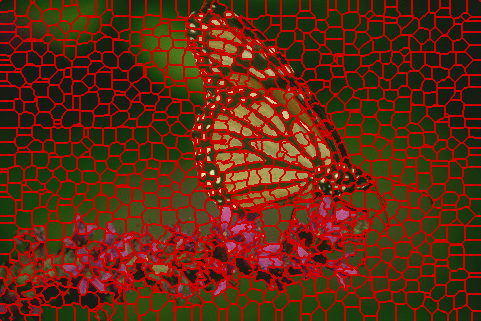
\includegraphics[width=9cm]{figuras/example-superpixel-segmentation}}
		}{
			\Fonte{\cite{SuperPixelBenchmark2017}}
		}
\end{figure}



Seguindo essa perspectiva, ao utilizar um algoritmo de extração de
\textit{features} de imagens sobre o superpixel, tem-se que o vértice
do grafo é neste momento um vetor de características. O sistema de
competição proposto no artigo \textit{Network Unfolding Map By
Vertex-Edge Dynamics Modeling} pode otimizar o pertencimento de
classes (segmentos, nesse caso) baseado na topologia de sua vizinhança
e na relação aos vértices conectados. A métrica de similaridade
(por exemplo, distância euclidiana, cosseno, etc.) pode ser
ajustada de acordo com o problema.

Ao considerar o problema como semi-supervisionado, a pista de ter
alguns dos superpixels anotados adicionaria um \textit{bias}
parametrizado pelo conhecimento do especialista em uso da ferramenta,
como um editor ou um médico. A otimização do pertencimento das classes
então seria acionada pela dinâmica coletiva selecionada em questão,
que, por acaso, poderia ser o algoritmo \gls{LCU} mencionado anteriormente.

Por outro lado, ainda há muitas melhorias a serem feitas nessas técnicas, como,
por exemplo: analisar as condições de convergência do algoritmo. Isso
pode ser um dos resultados deste trabalho, demandando uma análise
matemática com auxílio de experimentos.

É importante mencionar que já foi demonstrado em outras situações,
como em~\cite{JarbasComplexNetworks2020}, que o uso de redes complexas
em fusão com redes neurais aleatórias pode gerar um discriminante de
textura da imagem de alta relevância como extrator de
características. Neste caso, é possível se apoiar nesse resultado como
uma evidência de que a investigação de novas técnicas considerando a
topologia da imagem através de redes complexas é uma oportunidade de
pesquisa.


\subsection{GrabCut: Interactive Foreground Extraction Using Iterated
  Graph Cuts}\label{sec:grabcut}

Neste trabalho, um dos pioneiros em segmentação interativa, os
autores~\cite{rother2004grabcut} desenvolveram uma técnica para segmentação interativa
chamada GrabCut baseado em um mapeamento da imagem como um grafo e
então um corte entre as arestas é realizado para segmentar o objeto do
plano de fundo.


\subsection{Aplicação de agrupamento semi-supervisionado para segmentação
  de imagens coloridas}\label{sec:franciscolira2018}

Neste trabalho, o autor~\cite{franciscolira2018} na sua tese de
graduação, propõe variações de um algoritmo de segmentação de imagem
semi-supervisionado combinando algoritmos de agrupamento, como
\textit{Fuzzy C-Means}, Algoritmo de Pedrycs, Algoritmo
Semi-supervisionado Padrão (sSSC) e Algoritmo Semi-supervisionado
Regularizado por Entropia (ESSC).

\subsection{FocalClick: Towards Practical Interactive Image Segmentation}\label{sec:focalclick}

Neste trabalho, os autores~\cite{chen2022focalclick} criam uma técnica de
segmentação interativa em busca da praticidade, ao medir dois aspectos
importantes além de qualidade de segmentação: necessidade de anotação
e tempo de execução. O trabalho em sua metodologia de avaliação,
utiliza métricas para minimizar interações que o usuários tenha que
fazer para alcançar uma segmentação de qualidade. Essa técnica se
baseia num algoritmo iterativo que possui capacidades de correção ao
incluir novas marcações. Na Figura~\ref{fig:focalclick} é possível visualizar uma
visão geral da técnica:


\begin{figure}[!h]
        \captionsetup{width=12cm}
		\Caption{\label{fig:focalclick}
          Visão geral da técnica de segmentação interativa FocalClick.}
		\centering
		\UFCfig{}{
			\fbox{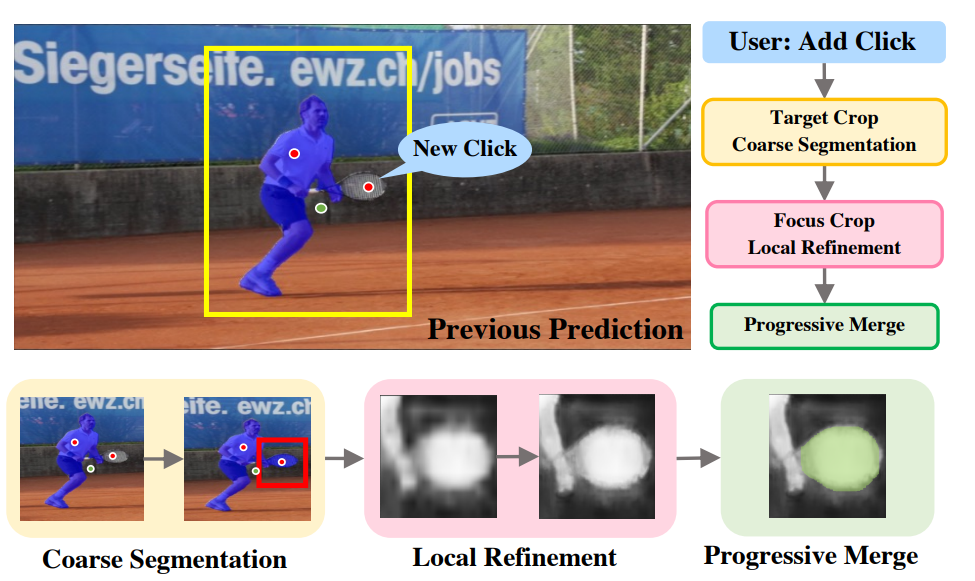
\includegraphics[width=12cm]{figuras/focalclick}}
		}{
			\Fonte{\cite{chen2022focalclick}}
		}
\end{figure}


\subsection{Interactive image segmentation based on multi-layer
random forest classifiers}\label{sec:superpixel-random-forest}

Neste trabalho, as autoras\cite{shan2023interactive} criam uma nova
técnica para segmentação interativa de imagens combinando uma
pré-segmentação usando superpixels e duas camadas de modelos random
forest para classificar o agrupamento entre os superpixels numa
máscara de segmentação resultante.


\section{Justificativas}\label{sec:justificativas}

Como mencionado na introdução, os algoritmos conhecidos de segmentação
de imagens possuem restrições pertinentes que podem dificultar o uso
das técnicas em alguns problemas, como imagens médicas e edição de
imagens.

Estes problemas são endereçados no desenvolvimento de uma nova técnica
de segmentação de imagens que explora outros novos ramos de
aprendizagem de máquina semi-supervisionada além das \gls{DNN}, neste
caso utilizando redes complexas e dinâmicas coletivas.

O campo de pesquisa de segmentação interativa também tem tido aumento
na publicação de artigos de relevância, em especial a publicação de
artigos com a palavra-chave GrabCut (tipo de algoritmo para
segmentação interativa), como pode ser visto na
Figura~\ref{fig:grabcut-papers}:

\begin{figure}[!h]
        \captionsetup{width=12cm}
		\Caption{\label{fig:grabcut-papers}
          Quantidade de publicações relevantes envolvendo grabcut de
          2004 a 2022}
		\centering
		\UFCfig{}{
			\fbox{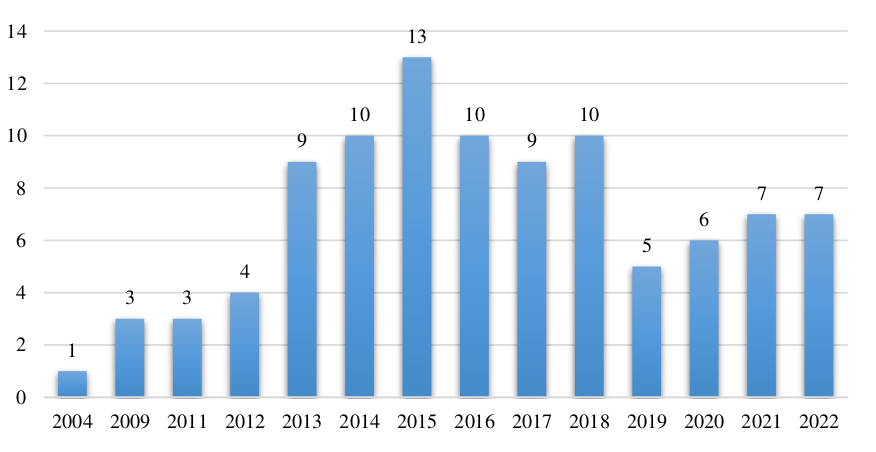
\includegraphics[width=12cm]{figuras/grabcut-papers}}
		}{
			\Fonte{\cite{wang2023review}}
		}
\end{figure}



\section{Objetivo Geral}\label{sec:objetivo-geral}

Desenvolver uma nova técnica de segmentação de imagens
semi-supervisionada que possa ser equiparável ao estado da arte, com
foco em segmentação interativa.

\section{Objetivos Específicos}\label{sec:objetivo-geral}

\begin{itemize}
\item Explorar técnicas de redes complexas e dinâmicas coletivas sobre
  o problema de segmentação de imagens.
\item Aplicar em casos variados de segmentação de imagens, como
  objetos comuns, carros.
\item Avaliar o impacto da segmentação por superpixel na segmentação final.
\item Desenvolver uma ferramenta para segmentação interativa
  utilizando o método de segmentação proposto.
\end{itemize}



% LocalWords:  transdutivo superpixel

	\chapter{OBJETIVOS}\label{cap:objetivos}

\begin{itemize}
\item Desenvolver uma nova técnica de segmentação de imagens que possa ser
equiparável ao estado da arte, como \textit{Mask R-CNN}, mas com menor
complexidade computacional e baixo número de anotação de dados.
\item Explorar técnicas de Redes Complexas e Dinâmicas Coletivas sobre
  o problema de segmentação de imagens.
\item Aplicar a técnica desenvolvida em casos de imagens médicas, como
  radiografias pulmonares.
\item Aplicar em casos variados de segmentação de imagens, como
  objetos comuns, carros.
\end{itemize}

	\chapter{Justificativas}\label{cap:justificativas}

Como mencionado na introdução, os algoritmos conhecidos de segmentação
de imagens possuem restrições pertinentes que podem dificultar o uso
das técnicas em alguns problemas, como imagens médicas e edição de
imagens. Na seção \textit{revisão biblográfica} são mencionadas propriedades
pertinentes dos algoritmos propostos, como, por exemplo, possuirem complexidade
computacional linear.

Estes problemas são endereçados no desenvolvimento de uma nova técnica
de segmentação de imagens que explora outros novos ramos de
aprendizagem de máquina semi-supervisionada além das \gls{DNN}, neste
caso utilizando redes complexas e dinâmicas coletivas. Parte do
trabalho que tem sido desenvolvido em parceria com o \gls{ITA} no
projeto DNAYA\cite{DnayaMotivation}, como por exemplo a dinâmica coletiva \gls{LCU}.

Vale mencionar que, considerando a situação de pandemia que vive-se
desde 2020 com o COVID-19, a construção de tecnologias que facilitam o
diagnóstico de doenças respiratórias com auxílio de radiografias
pulmonares tem se tornado uma linha de pesquisa ainda mais relevante.

	\chapter{Revisão Bibliográfica}\label{cap:revisao-bibliografica}

Técnicas de segmentação de imagens com o paradigma semi-supervisionado
estão em foco atualmente no campo médico, como pode ser visto em
\cite{LuoSemiSupervised2021}. Nesse artigo, uma das grandes motivações
de os autores utilizarem uma técnica semi-supervisionada
está relacionado com a dificuldade de anotação de dados no ambiente
hospitalar, requisito para utilizar técnicas mais robustas como
\textit{Mask R-CNN}.

Em relação ao tópico de redes complexas e dinâmicas coletivas, é
possível mencionar o trabalho feito com o algoritmo \gls{LCU}
\cite{VerriNetworkUnfoldingMap2018} no qual os principais conceitos
sobre resolução de problemas de aprendizagem de máquina
semi-supervisionada são explorados em detalhes como uma dinâmica de
competição de partículas na relação vértice-arestas de um grafo
não-direcionado. Este método de aprendizagem é transdutivo, portanto,
difere dos métodos indutivos, como é o caso de Redes Neurais. Além
disso, esse algoritmo tem complexidade computacional linear em relação
à quantidade de classes, arestas e vértices.

Para ilustrar uma possível ideia de segmentação de imagens, ao
considerar um algoritmo que faça uma transformação do domínio de imagem para um
grafo, é possível estabelecer uma relação na qual os vértices representam
parte da imagem como um \textit{superpixel}
\cite{SuperpixelSurvey2020}, ou seja, um grupo de subpixels da
imagem. Algoritmos de superpixel são não-supervisionados em geral,
portanto possuem suas limitações quanto ao resultado esperado pelo
usuário \textendash \hfill logo difícil de ser aceito em aplicações médicas
nas quais a opinião do especialista é de alta relevância para o
resultado final.

\begin{figure}[!h]
        \captionsetup{width=9cm}
		\Caption{\label{fig:segmentation-superpixel}
          Segmentação superpixel}
		\centering
		\UFCfig{}{
			\fbox{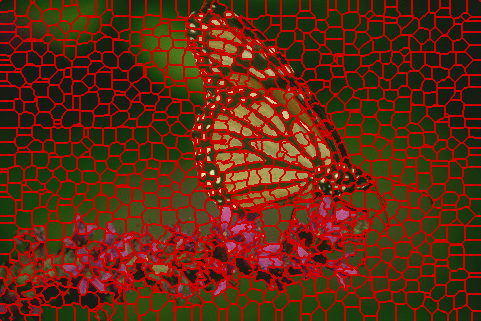
\includegraphics[width=9cm]{figuras/example-superpixel-segmentation}}
		}{
			\Fonte{\cite{SuperPixelBenchmark2017}}
		}
\end{figure}



Seguindo essa perspectiva, ao utilizar um algoritmo de extração de
\textit{features} de imagens sobre o superpixel, tem-se que o vértice
do grafo é neste momento um vetor de características. O sistema de
competição proposto no artigo \textit{Network Unfolding Map By
Vertex-Edge Dynamics Modeling} pode otimizar o pertencimento de
classes (segmentos, nesse caso) baseado na topologia de sua vizinhança
e na relação aos vértices conectados. A métrica de similaridade
(por exemplo, distância euclidiana, cosseno, etc.) pode ser
ajustada de acordo com o problema.

Ao considerar o problema como semi-supervisionado, a pista de ter
alguns dos superpixels anotados adicionaria um \textit{bias}
parametrizado pelo conhecimento do especialista em uso da ferramenta,
como um editor ou um médico. A otimização do pertencimento das classes
então seria acionada pela dinâmica coletiva selecionada em questão,
que, por acaso, poderia ser o algoritmo \gls{LCU} mencionado anteriormente.

Por outro lado, ainda há muitas melhorias a serem feitas nessas técnicas, como,
por exemplo: analisar as condições de convergência do algoritmo. Isso
pode ser um dos resultados deste trabalho, demandando uma análise
matemática com auxílio de experimentos.

É importante mencionar que já foi demonstrado em outras situações,
como em \cite{JarbasComplexNetworks2020}, que o uso de redes complexas
em fusão com redes neurais aleatórias pode gerar um discriminante de
textura da imagem de alta relevância como extrator de
características. Neste caso, é possível se apoiar nesse resultado como
uma evidência de que a investigação de novas técnicas considerando a
topologia da imagem através de redes complexas é uma oportunidade de
pesquisa.

% LocalWords:  transdutivo superpixel

	\chapter{Metodologia}\label{cap:metodologia}


Este trabalho de conclusão de concurso será dividido em quatro fases:
Pesquisa, Desenvolvimento, Testes e Monografia.

Durante a pesquisa científica, os artigos referenciados serão explorados com
maior atenção e será buscado entender os detalhes que implicam
na criação da técnica proposta. Em especial, dois artigos terão maior
atenção inicialmente: \textit{Network Unfolding Map By Vertex-Edge
  Dynamics Modeling} \cite{VerriNetworkUnfoldingMap2018} e
\textit{Image Segmentation Methods Based on Superpixel Techniques A
  Survey} \cite{SuperpixelSurvey2020}. O primeiro contém a definição
da técnica LCU, uma dinâmica coletiva sobre redes complexas, o
componente de aprendizagem principal do algoritmo; o segundo será
usado como uma pré-segmentação inicial antes de partir pra construção
da rede complexa. Na figura \ref{fig:fluxograma-algoritmo} é demonstrada uma
visão macro do algoritmo.

\begin{figure}[!h]
        \captionsetup{width=8cm}
		\Caption{\label{fig:fluxograma-algoritmo}
          Algoritmo de segmentação semi-supervisionada de imagens}
		\centering
		\UFCfig{}{
			\fbox{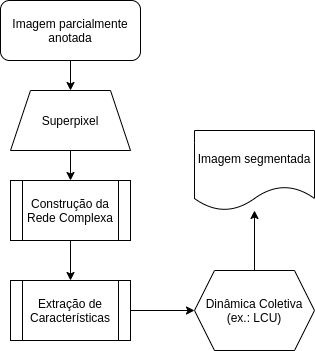
\includegraphics[width=8cm]{figuras/algorithm}}
		}{
			\Fonte{Autoral}
		}
\end{figure}


O desenvolvimento se concentrará na integração das técnicas
mencionadas acima como uma nova técnica de segmentação de imagens
semi-supervisionada, portanto, serão detalhadadas todas as
etapas necessárias pra construção e aplicação do novo algoritmo de
segmentação. Por exemplo, a construção da rede complexa assumirá
que cada superpixel será um vértice do grafo com seus vizinhos baseado
na topologia da imagem, a etapa de extração de características
ocorrerá em cada superpixel e a dinâmica coletiva considerará a
anotação parcial da imagem. No fim do algoritmo, os segmentos da
imagem serão subgrafos dessa rede complexa.

Adicionalmente, a implementação do algoritmo nesse trabalho será
construída de maneira \textit{Open Source} como uma ferramenta de
simulação de segmenteção, usando a biblioteca \gls{OpenCV} para que possa
ser testado o algoritmo de segmentação de imagens recebendo pontos
aleatórios de marcação do usuário. Isto simulará o caso de um
especialista analisando uma imagem médica, por exemplo.


Na fase de testes, a avaliação dos resultados considerará os
principais \textit{datasets} conhecidos para segmentação de imagens,
como o \textit{The Berkeley Segmentation Dataset and Benchmark}
\cite{MartinFTM01}.

Na fase de monografia serão consolidados todos os resultados em um
trabalho acadêmico nas normas da \gls{ABNT}.

O cronograma das atividades de pesquisa é apresentado a seguir.

\begin{table}[h]
\begin{tabular}{l|l|l|l|l|l|l|}
\cline{2-7}
                                          & Abril                                         & Maio                                            & Junho                                           & Julho                                           & Agosto                                          & Setembro                                        \\ \hline
\multicolumn{1}{|l|}{Pesquisa científica} & \multicolumn{1}{c|}{\cellcolor[HTML]{000000}} & \cellcolor[HTML]{000000}{\color[HTML]{000000} } & \cellcolor[HTML]{000000}{\color[HTML]{000000} } &                                                 &                                                 &                                                 \\ \hline
\multicolumn{1}{|l|}{Desenvolvimento}     &                                               &                                                 & \cellcolor[HTML]{000000}{\color[HTML]{000000} } & \cellcolor[HTML]{000000}{\color[HTML]{000000} } &                                                 &                                                 \\ \hline
\multicolumn{1}{|l|}{Testes}              &                                               &                                                 &                                                 & \cellcolor[HTML]{000000}{\color[HTML]{000000} } & \cellcolor[HTML]{000000}{\color[HTML]{000000} } &                                                 \\ \hline
\multicolumn{1}{|l|}{Monografia}          &                                               &                                                 &                                                 &                                                 & \cellcolor[HTML]{000000}{\color[HTML]{000000} } & \cellcolor[HTML]{000000}{\color[HTML]{000000} } \\ \hline
\end{tabular}
\end{table}


	%Elementos pós-textuais
	\bibliography{3-pos-textuais/referencias}
%	\imprimirglossario
	% \imprimirapendices
	% 	% Adicione aqui os apendices do seu trabalho
	% 	\apendice{Exemplo de apêndice}
\label{ap:A}

Um apêndice é um documento elaborado pelo autor, diferentemente do anexo. Geralmente, se coloca como apêndice, questionários, códigos de programação, tabelas que tomariam muito espaço no meio do trabalho. Artigos, resumos ou qualquer publicação relacionada ao trabalho podem ser utilizados como apêndice.
	% 	\apendice{Questionário utilizado para...}
\label{ap:B}

\begin{questao}
	\item Esta é a primeira questão com alguns itens:
		\begin{enumerate}
			\item Este é o primeiro item
			\item Segundo item
		\end{enumerate}
	\item Esta é a segunda questão:
		\begin{enumerate}
			\item Este é o primeiro item
			\item Segundo item
		\end{enumerate}
	\item Lorem ipsum dolor sit amet, consectetur adipiscing elit. Nunc dictum sed tortor nec viverra. consectetur adipiscing elit. Nunc dictum sed tortor nec viverra.
		\begin{enumerate}
			\item consectetur
			\item adipiscing
			\item Nunc
			\item dictum
		\end{enumerate}
\end{questao}

	% 	\apendice{Códigos-fontes utilizados para...}
\label{ap:C}

\lstinputlisting[language=C++,caption={Hello World em C++}]{figuras/main.cpp}


\begin{lstlisting}[language=Java,caption={Hello World em Java}]
public class HelloWorld {
	public static void main(String[] args) {
		System.out.println("Hello World!");
	}
}
\end{lstlisting}


	% 	\apendice{\textit{IEEE CEFC 2016}}
\label{ap:D}

\textit{Digest} submetido ao \textit{The 17th Biennial Conference on Eletromagnetic Field Computation, Miami FL - NOV 13-16, 2016, USA}.

%Código fonte para inserir um arquivo em PDF
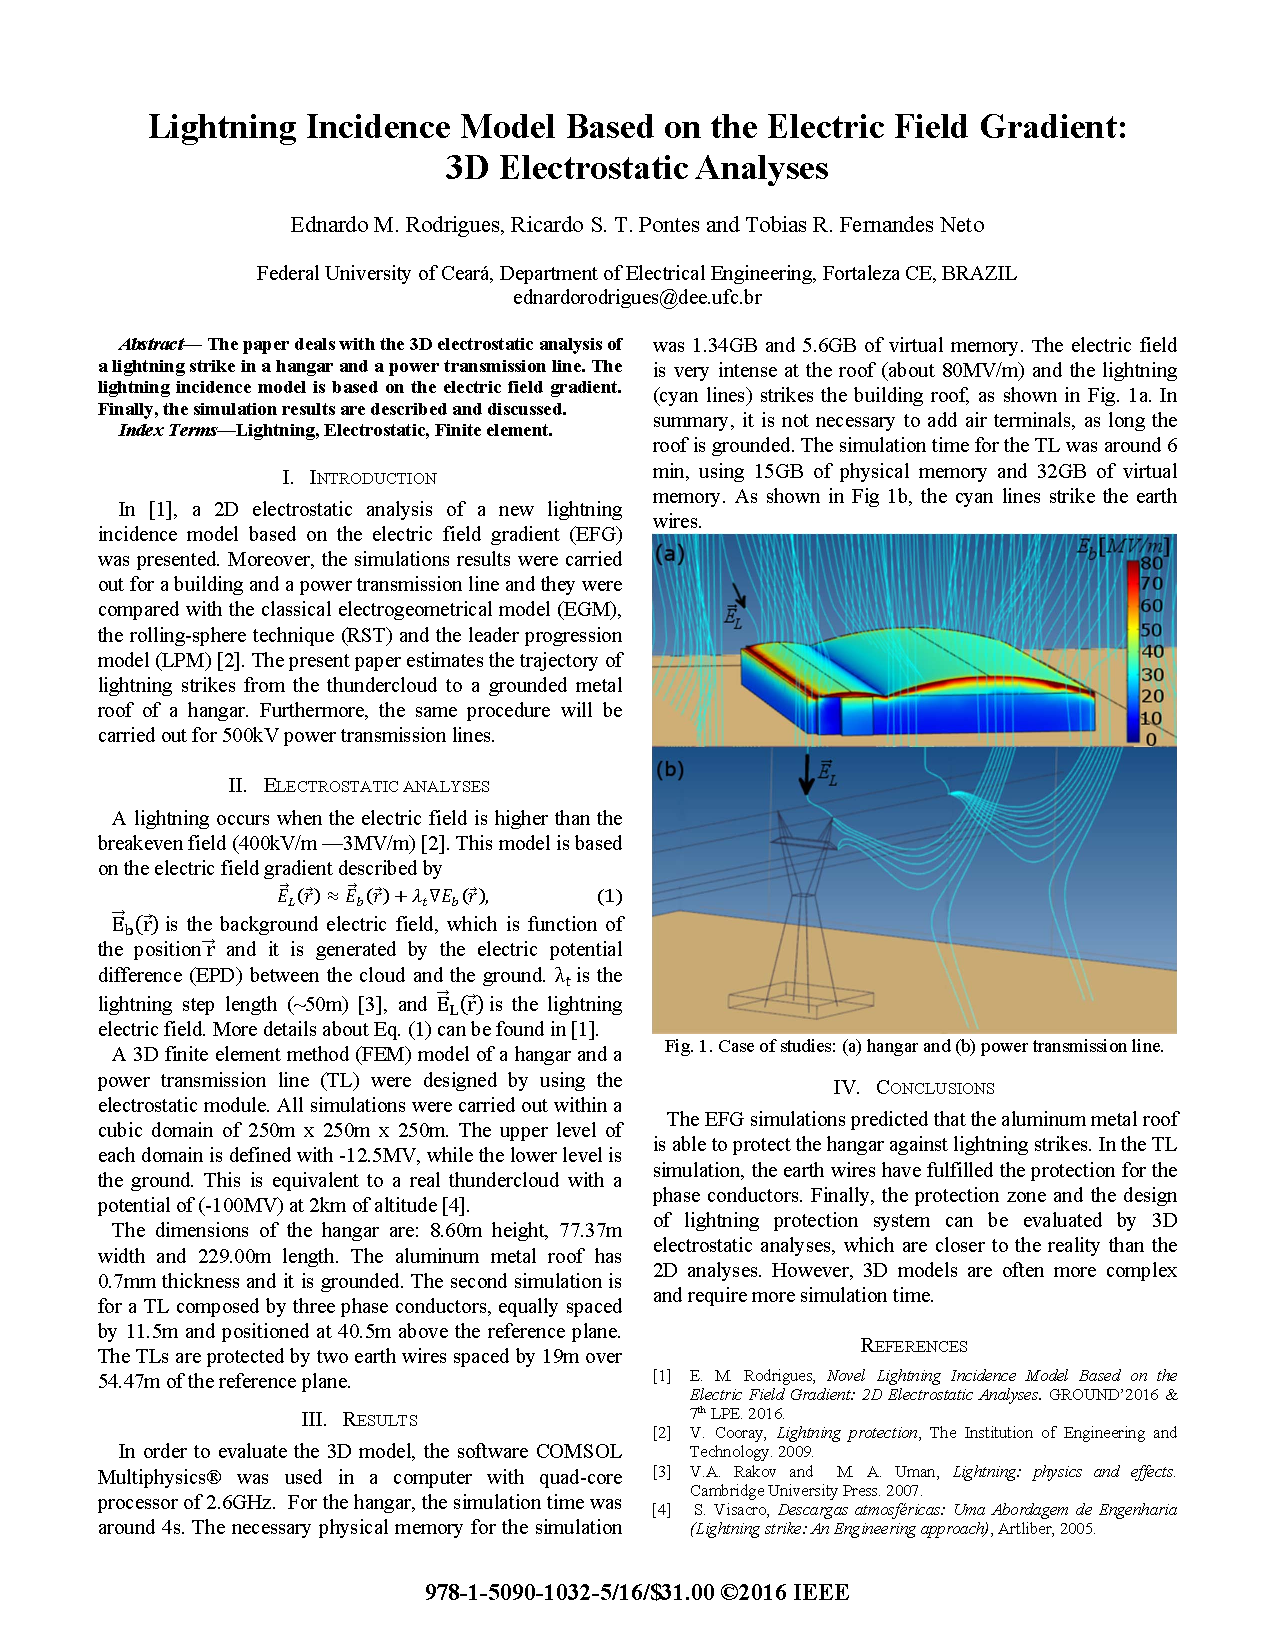
\includepdf[pages={-}]{3-pos-textuais/apendices/PID4416093.pdf}
	% \imprimiranexos
	% 	% Adicione aqui os anexos do seu trabalho
	% 	\anexo{Exemplo de um anexo}
\label{an:ex_anexo_a}

Um anexo é um documento que não foi elaborado pelo autor, ou seja, o autor apenas anexa. Anexos podem ser tabelas, mapas, diagramas, \textit{datasheets}, manuais e etc. 




	% 	\anexo{Exemplo de um anexo em PDF}
\label{an:ex_anexo_b}

O autor pode anexar um \gls{PDF}, traduzido como formato portátil de documento. Veja o código fonte utilizado para anexar o arquivo ``Sikasil.pdf'' que foi colocado dentro da pasta ``anexos'' que por sua vez está dentro da pasta ``elementos-pos-textuais''. Tenha muita atenção na hora de especificar o local do arquivo. Recomenda-se não utilizar caracteres especiais para nomear pastas e, principalmente, arquivos. 

Pode-se fazer uma descrição sucinta do arquivo anexado.

%Comando para incluir um arquivo em PDF:
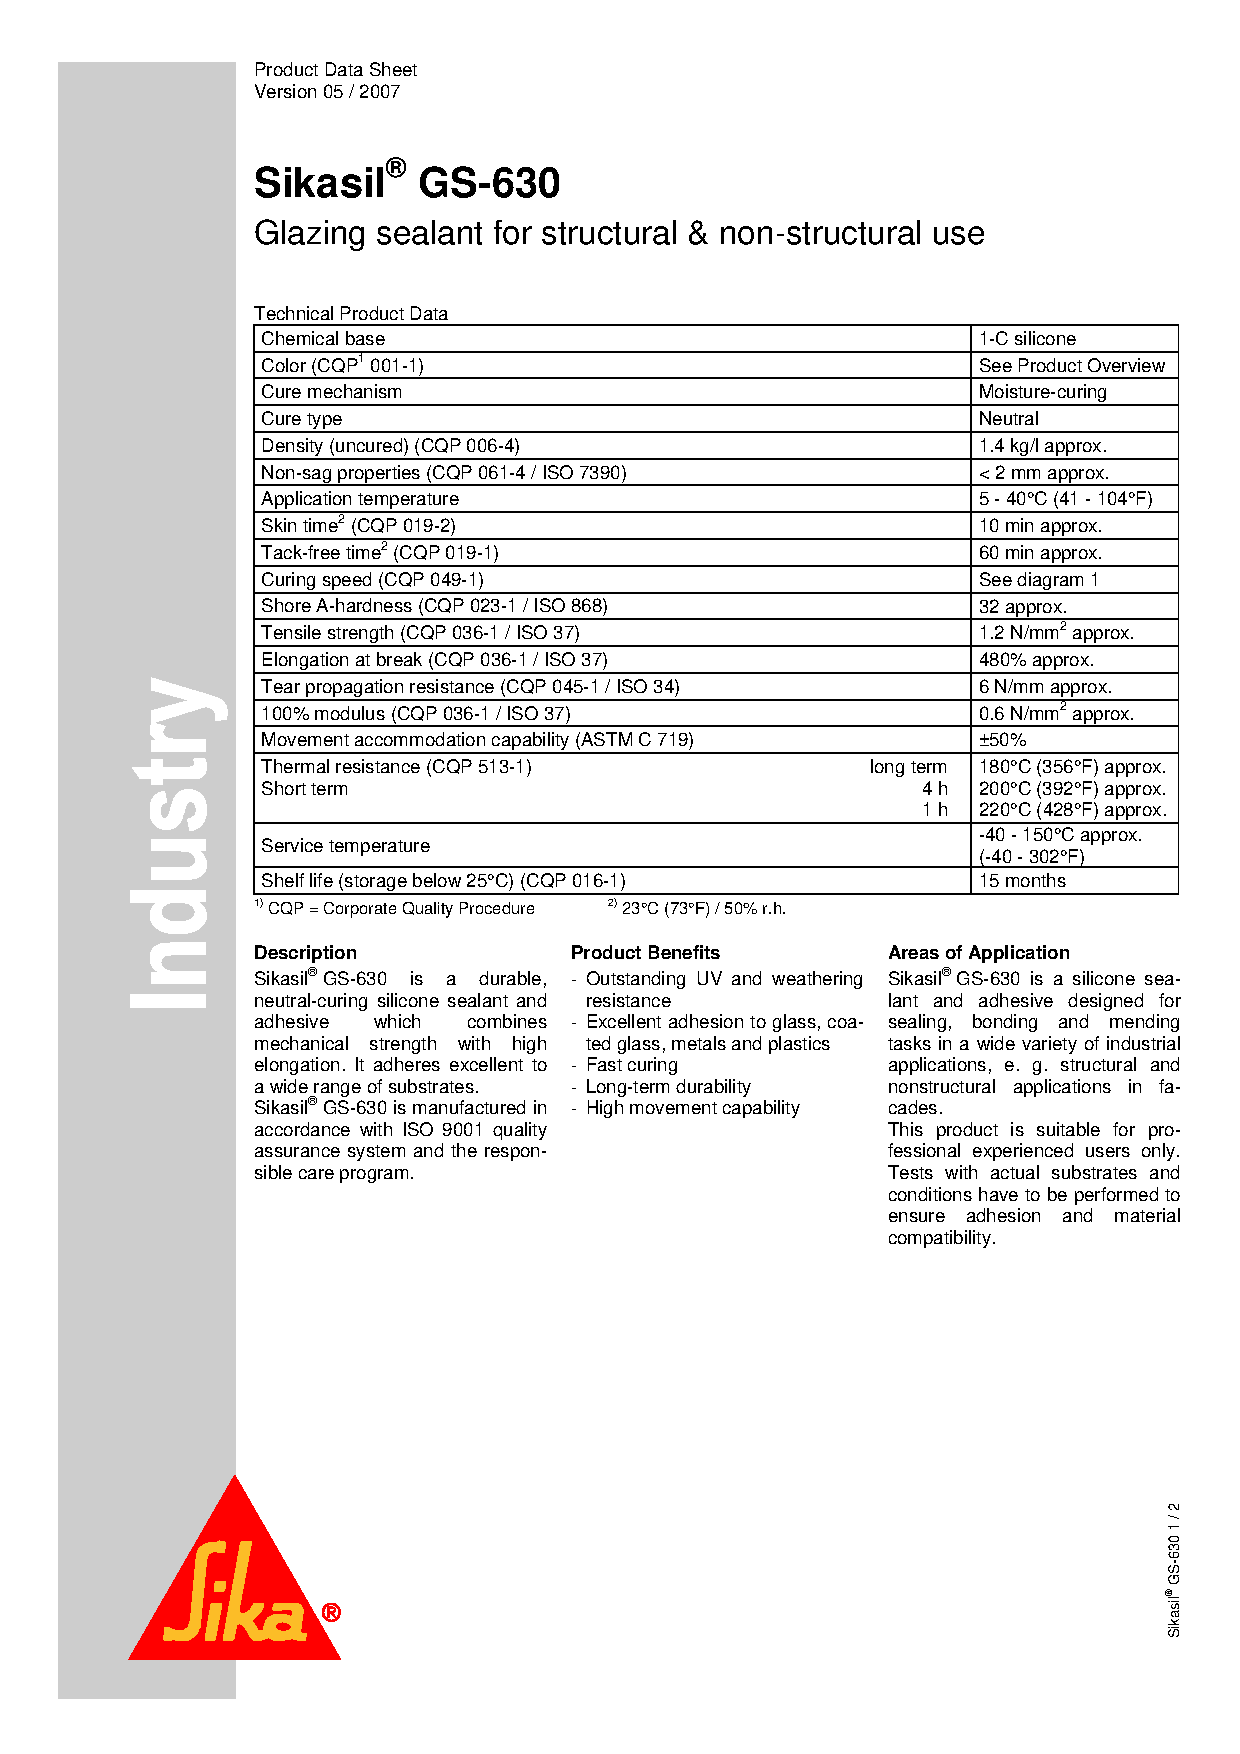
\includepdf[pages={-}]{3-pos-textuais/anexos/Sikasil.pdf}


	% \imprimirindice

\end{document}
